% Figura Anexo II: efectos riqueza en el IS-LM: (a) política monetaria expansiva; (b) política fiscal expansiva con deuda
\documentclass[tikz,border=3pt]{standalone}
\usepackage[T1]{fontenc}
\usepackage[utf8]{inputenc}
\usetikzlibrary{arrows.meta,calc,positioning}
\begin{document}
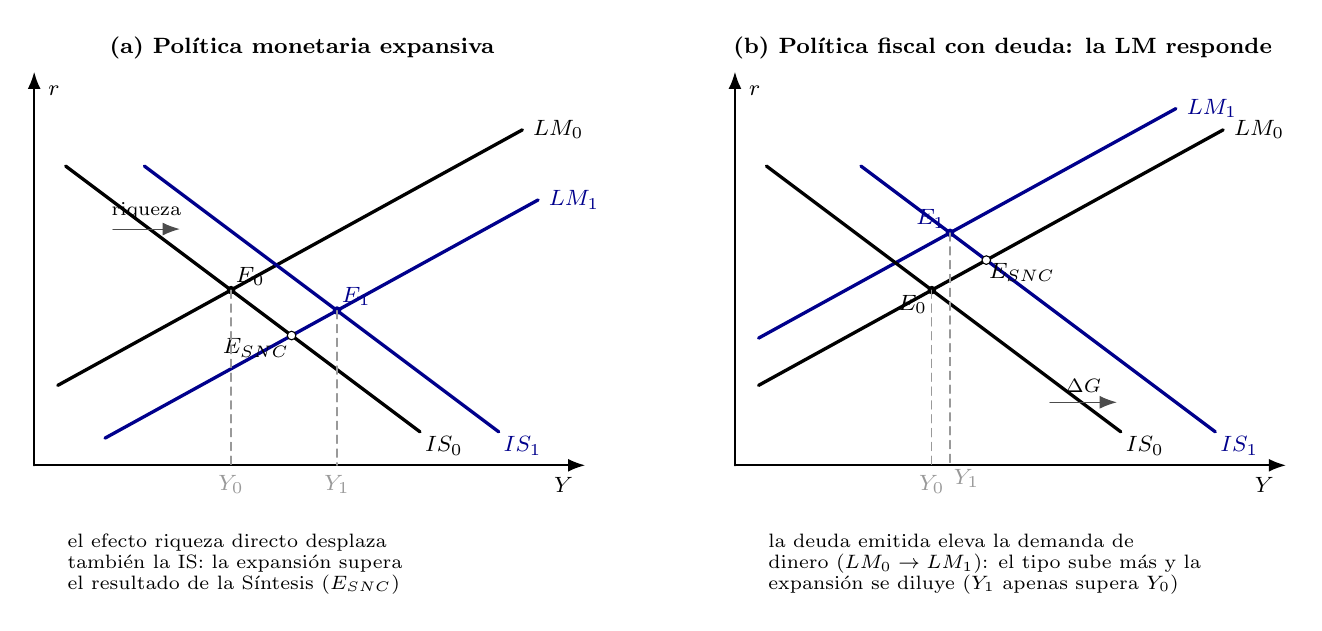
\begin{tikzpicture}[>={Latex[length=2.2mm]}, line cap=round, font=\footnotesize,
  eje/.style={->, thick},
  curva/.style={very thick},
  nueva/.style={very thick, blue!55!black},
  guia/.style={densely dashed, gray!80},
  pto/.style={circle, fill=black, inner sep=1.1pt}]
  % ---------- Panel (a): política monetaria ----------
  \node[font=\footnotesize\bfseries] at (3.4,5.3) {(a) Política monetaria expansiva};
  \draw[eje] (0,0) -- (7.0,0) node[below left=1pt]{$Y$};
  \draw[eje] (0,0) -- (0,5.0) node[below right=2pt]{$r$};
  \draw[curva] (0.3,1.015) -- (6.2,4.26) node[right]{$LM_0$};
  \draw[nueva] (0.9,0.345) -- (6.4,3.37) node[right]{$LM_1$};
  \draw[curva] (0.4,3.80) -- (4.9,0.425) node[below right=-3pt]{$IS_0$};
  \draw[nueva] (1.4,3.80) -- (5.9,0.425) node[below right=-3pt]{$IS_1$};
  \draw[->, gray!60!black] (1.0,3.0) -- (1.85,3.0) node[midway, above=0pt, black]{\scriptsize riqueza};
  \node[pto] (A0) at (2.5,2.225) {};
  \node[above right=-1pt of A0, inner sep=1pt] {$E_0$};
  \node[circle, draw=black, fill=white, inner sep=1.1pt] (As) at (3.269,1.648) {};
  \node[below left=-2pt of As, inner sep=1pt] {$E_{SNC}$};
  \node[pto, fill=blue!55!black] (A1) at (3.846,1.965) {};
  \node[above right=-1pt of A1, inner sep=1pt, blue!55!black] {$E_1$};
  \draw[guia] (2.5,2.225) -- (2.5,0) node[below]{$Y_0$};
  \draw[guia] (3.846,1.965) -- (3.846,0) node[below]{$Y_1$};
  \node[align=left, anchor=north west] at (0.3,-0.75) {\scriptsize el efecto riqueza directo desplaza\\[-2pt]\scriptsize también la IS: la expansión supera\\[-2pt]\scriptsize el resultado de la Síntesis ($E_{SNC}$)};
  % ---------- Panel (b): política fiscal ----------
  \begin{scope}[xshift=8.9cm]
    \node[font=\footnotesize\bfseries] at (3.4,5.3) {(b) Política fiscal con deuda: la LM responde};
    \draw[eje] (0,0) -- (7.0,0) node[below left=1pt]{$Y$};
    \draw[eje] (0,0) -- (0,5.0) node[below right=2pt]{$r$};
    \draw[curva] (0.3,1.015) -- (6.2,4.26) node[right]{$LM_0$};
    \draw[nueva] (0.3,1.615) -- (5.6,4.53) node[right]{$LM_1$};
    \draw[curva] (0.4,3.80) -- (4.9,0.425) node[below right=-3pt]{$IS_0$};
    \draw[nueva] (1.6,3.80) -- (6.1,0.425) node[below right=-3pt]{$IS_1$};
    \draw[->, gray!60!black] (4.0,0.8) -- (4.85,0.8) node[midway, above=0pt, black]{\scriptsize $\Delta G$};
    \node[pto] (B0) at (2.5,2.225) {};
    \node[below left=-1pt of B0, inner sep=1pt] {$E_0$};
    \node[circle, draw=black, fill=white, inner sep=1.1pt] (Bs) at (3.192,2.606) {};
    \node[below right=-2pt of Bs, inner sep=1pt] {$E_{SNC}$};
    \node[pto, fill=blue!55!black] (B1) at (2.731,2.952) {};
    \node[above left=-1pt of B1, inner sep=1pt, blue!55!black] {$E_1$};
    \draw[guia] (2.5,2.225) -- (2.5,0) node[below]{$Y_0$};
    \draw[guia] (2.731,2.952) -- (2.731,0) node[below right=-3pt]{$Y_1$};
    \node[align=left, anchor=north west] at (0.3,-0.75) {\scriptsize la deuda emitida eleva la demanda de\\[-2pt]\scriptsize dinero ($LM_0\to LM_1$): el tipo sube más y la\\[-2pt]\scriptsize expansión se diluye ($Y_1$ apenas supera $Y_0$)};
  \end{scope}
\end{tikzpicture}
\end{document}
